\chapter{The research: Development of a flight simulation model}

This chapter will focus on the work performed during the internship. It starts defining the main task and goals of the project and continues with a description of the methodology used. Then it focuses of the work done during the internship and finishes by presenting the end results.

\section{Problem statement}
Currently DAWN has began with the flight tests of their first research vehicle. As development is progressing the need for research into the \gls{cns} is growing. An important part in the development of these system are the flight models needed to tune controllers, aircraft design, systems software and hardware in the loop tests, etc. 

\subsection{Problem analysis and definition}
The development of these flight models is not easy, with the main problem being determining the aerodynamic properties of the aircraft. There are several options for determining the aerodynamic coefficients, each one with the own advantages and disadvantages.

\begin{itemize}
\item \textbf{Empirical models} \\ It is possible to get an estimate of the aerodynamic coefficients by using empirical models and tools. The advantage of these models is that they can quickly determine the aerodynamic coefficients for a wide range of flight conditions. However these tools are not accurate and can only be used for the early design stages.

\item \textbf{Computational models} \\ Another option is to calculate these coefficients based on numerical methods such as \gls{cfd} or potential flow. The main advantage is that they will give more accurate results than the empirical models and since no physical model is needed it's possible to change the design in order to optimize its flight characteristics. The disadvantages are that these methods can be computationally intensive and require special knowledge in order to perform them correctly.

\item \textbf{Wind tunnel} \\
Wind tunnel tests can give accurate estimates on the aerodynamic properties of the aircraft and since no full sized aircraft is needed it is still possible to perform changes to the aircraft. However wind tunnel availability and the limited number of flight conditions in which wind tunnel tests can be performed are the main problems.

\item \textbf{Real flight system identification} \\
The aerodynamic properties of the aircraft can also be determined using measurements taken during real flights. The main advantage is that if done correctly, these methods will give the most accurate estimate of the aerodynamic properties of the aircraft, which will give the information necessary to optimize the control systems. The main drawbacks are that a flight capable model is needed and the limited amount of flight data that can be collected.
\end{itemize}

Thus the main problem to be solved is: How can an accurate flight model be created with the resources currently available within DAWN.

\subsection{Goal and end product}
The end goal of the project is to research into the development of the tools necessary to create accurate flight simulation models. The end product will be a set of basic tools demonstrating the steps that need to be taken and a list of recommendations for the further development of these tools.

\section{Methodology}

\section{Work performed}
\subsection{Introduction and familiarization with the company and project}
The first step was to gain knowledge on the development that had already been done within DAWN, gather information on the current equipment and familiarize with the tools available.

\subsubsection{Current equipment}
The main flight computer being used on the current vehicle is the Pixhawk 2 running the Ardupilot autopilot software. The Pixhawk 2 is an open source flight computer designed by the Pixhawk open hardware community and thanks to its integrated sensors, redundant hardware and compact design it provides all the basic hardware needed to safely fly a small to medium sized drone. Ardupilot is a well developed open source autopilot software, it fully supports the Pixhawk 2 and provides the control, state estimation and navigation software needed to fly the current flight vehicle.

\subsubsection{Familiarization tasks}
Since the to be developed modeling tools would eventually have to be used with the Pixhawk and interface with Ardupilot two tasks where performed in order to familiarize with Ardupilot. The first tasks was the addition of new telemetry packages to the Ardupilot telemetry system. During this task basic knowledge was collected on the structure of the Ardupilot software and how to modify it. \\

The second task was setting up a \gls{sitl} test setup. This consisted of running the Ardupilot software on a development computer, in this case a laptop, and connect its sensor input, control outputs and telemetry outputs to a \gls{fdm} and a ground station software running on the same computer. The purpose of this setup is to provide an environment in which modifications to the Ardupilot software can be rapidly and safely tested without the need of the hardware. This allows the use of advanced software development tools that are not available for embedded systems, greatly simplifying the software development process without putting any of the equipment at risk. \\

Ardupilot's \gls{sitl} software package gives a wide range of options when it comes to the \gls{fdm} programs it can be connected to. Since further development of the simulation model synthesizing tools would depend on the \gls{fdm} chosen during this task a small trade-of was made to choose the appropriate tool for this stage of the project. The main points of interest for the \gls{fdm} where that it had to be easy to interface with from external software, easy to extend with new features, stable and accurate. \\

In the end JSBSim was chosen. JSBSim is an open source \gls{fdm} software library capable of modeling a wide range of aerospace vehicles. It's used by many open source flight simulation software packages most notably Flightgear and OpenEaagles and has been used on several university research projects around the world. The latest release contains all the features that will be necessary for the foreseeable future and its designed allows it to be easily extended or incorporated into other software tools. This is also the default \gls{fdm} for the Ardupilot SILT software and is thus the best supported one.

\subsection{Plan of approach}
After completing the familiarization tasks a plan of approach was made. As mentioned in the problem statement there are several options when it comes to determining the aerodynamic coefficients necessary to create the flight models. Wind tunnel tests and \gls{cfd} are not an option due to the limited time frame of the internship and the lack of expertise necessary to perform these. This leaves the empirical methods and system identification. \\

Empirical tools are able to quickly give an estimate of the aerodynamic coefficients, however these will be inaccurate and it is necessary to correct them if they will be used to design the control systems. Aerodynamic models based the system identification of real flight data are more accurate, but since this requires the aircraft to be physically flown, it limits the amount of flight data that can be collected, and thus the number of flight conditions at which the aerodynamic properties can be determined. \\

Thus the plan of approach is to combine both methods. The empirical tools will be used to create a large set of \textit{cheap} coefficients for a wide range of flight conditions and the \textit{expensive} coefficients will be determined with system identification of real flight data. This means that a tool to combine the two sets of coefficients will have to be developed.\\

Since the focus for now will be on the development of these tools. It is necessary to have a set of flight data for which the correct aerodynamic model is known. The easiest way to get such data is to calculate it using a simulation. Thus JSBSim will be used to generate this test data.\\

Digital Datcom is a freely available program capable if calculating the aerodynamic coefficients using empirical method, It is used to create the aerodynamic models used to develop the rest of the tools.\\

The two step approach is chosen as the system identification method. The first step is the state reconstruction step. Here sensor errors are determined and corrected and unmeasurable states are estimated. The next step is the parameter estimation step. Here the model structure is selected and the parameters of the chosen model are estimated 

\subsection{3rd party tools interface development}
To limit the amount of work necessary to complete these tasks, some third party software packages will be used. However since the to be developed tools will be written in Python it's necessary to make sure it is possible to interface with these tools from within a python script. The programs that will need interfaces are JSBSim and Digital Datcom.

\subsubsection{JSBSim}
JSBSim is an open-source \gls{fdm} software library written in C++ and by default provides no python bindings. So the first step was to look for existing python interfaces. The search revealed two possible options, "JSBSim Python" and "PyJSBSim". \\

Since the Sourceforge website was down at the time, the developer of "JSBSim Python" was directly contacted in order to get a copy of the source code and documentation. This revealed that the library had not been updated since 2007 and that it would probably require modifications in order to make it run with the current versions of JSBSim and Python. \\

Development for PyJSBSim is not active either, but the JSBSim development team uses it as part of their unit tests. Thus the copy of PyJSBSim in the JSBSim code repository is guaranteed to work with the current version of JSBSim. However PyJSBSim only implements a small subset of the JSBSim API and it doesn't give the option to create new aircraft models from within python since these consists of \gls{xml} files that need to be manually created before running the simulation. \\

Thus the next step was to extend PyJSBSim to include the extra features that would be needed and create a set of functions capable of creating the JSBSim aircraft model \gls{xml} files. PyJSBSim is written in Cython, a static compiler for Python and the extended Cython programming language. Code written in Cython can seamlessly interact with C/C++ and Python code, making it the perfect tool to write interfaces between Python and C++ code. \\

The first modifications where to make PyJSBSim run properly in Python 3. The code was already running, but because of changes in the language some extra type conversions where necessary in order to make the Python side of the interface easier to work with. One important feature that had to be added was the ability to give JSBSim tables with predetermined the control inputs. The rest of the changes made to PyJSBSim consisted of exposing a few more C++ functions and classes to Python and annotating the Cython code with type information.\\

As mentioned before, a tool had to be developed in order to to create the JSBSim aircraft models from within Python code. Since the input files contain \gls{xml} code, Jinja2, a templating language for Python, was chosen to write \gls{xml} template files that could then be filled in from the python code. \\

However before development of this tool could start, the aerodynamic model had to be defined. The reason for this is because JSBSim does not have an aerodynamic model. Instead the equations to calculate the aerodynamic forces need to be given in the input \gls{xml} files. To keep it simple, the linear model described in the TU Delft Flight dynamics course was used as the basis \cite{fdreader}. \\

The aerodynamic forces and moments are calculated using equations \autoref{eq:f_a} and \autoref{eq:m_a}. The aerodynamic coefficients in the body reference frame are defined in \autoref{eq:body_coefs} and the dimensionless rates used in \autoref{eq:body_coefs} are defined in \autoref{eq:dim_less_rates}.

\begin{equation}
\label{eq:f_a}
{F_A} = \frac{1}{2}\rho V_{tas}^2S\left[ {\begin{array}{*{20}{c}}
{{C_X}}\\
{{C_Y}}\\
{{C_Z}}
\end{array}} \right]\\
\end{equation}

\begin{equation}
\label{eq:m_a}
{M_A} = \frac{1}{2}\rho {V^2}S\left[ {\begin{array}{*{20}{c}}
{{C_l} \cdot b}\\
{{C_m} \cdot \bar c}\\
{{C_n} \cdot b}
\end{array}} \right]
\end{equation}

\begin{equation}
\label{eq:body_coefs}
\arraycolsep=1.4pt\def\arraystretch{2.2}
\begin{array}{l}
{C_X} = C_{{X_0}} + ({C_{{X_u}}} - 2\;{C_{{X_0}}})\;\hat u + {C_{{X_\alpha }}}\alpha  + {C_{{X_{{\alpha ^2}}}}}{\alpha ^2} + C_{{X_{\dot{\alpha}}}}\hat{\dot{\alpha}}  + {C_{{X_q}}}\hat q + {C_{{X_{{\delta _e}}}}}{\delta _e}\\
{C_Y} = {C_{{Y_\beta }}}\beta  + {C_{{Y_p}}}\hat p + {C_{{Y_r}}}\hat r + {C_{{Y_{{\delta _a}}}}}{\delta _a} + {C_{{Y_{{\delta _r}}}}}{\delta _r}\\
{C_Z} = ({C_{{Z_u}}} - 2\;{C_{{Z_o}}})\;\hat u + {C_{{Z_\alpha }}}\alpha  + {C_{{Z_{\dot{\alpha}}}}\hat{\dot{\alpha}} + {C_{{Z_q}}}\hat q + C_{{Z_{{\delta _e}}}}}{\delta _e}\\
{C_l} = {C_{{l_\beta }}}\beta  + {C_{{l_p}}}\hat p + {C_{{l_r}}}\hat r + {C_{{l_{{\delta _a}}}}}{\delta _a} + {C_{{l_{{\delta _r}}}}}{\delta _r}\\
{C_m} = {C_{{m_u}}}\hat u + {C_{{m_\alpha }}}\alpha  + C_{{m_{\dot{\alpha}}}}\hat{\dot{\alpha}}  + {C_{{m_q}}}\hat q + {C_{{m_{{\delta _e}}}}}{\delta _e}\\
{C_n} = {C_{{n_\beta }}}\beta  + {C_{{n_p}}}\hat p + {C_{{n_r}}}\hat r + {C_{{n_{{\delta _a}}}}}{\delta _a} + {C_{{n_{{\delta _r}}}}}{\delta _r}
\end{array}
\end{equation}

\begin{equation}
\label{eq:dim_less_rates}
\arraycolsep=1.4pt\def\arraystretch{2.2}
\begin{array}{l}
\hat u = \frac{{u - V}}{V}\\
\hat{\dot{\alpha}} = \frac{\dot{\alpha}\bar{c}}{V}\\
\hat p = \frac{{pb}}{{2V}}\\
\hat q = \frac{{q\bar c}}{V}\\
\hat r = \frac{{pb}}{{2V}}
\end{array}
\end{equation}

Since the aircraft is assumed to be trimmed at the beginning of the simulation, It is assumed that the thrust equals the aerodynamic drag. Thus the thrust and the aerodynamic force coefficient term $C_{x_0}$ cancel each other out. The $C_{x_0}$ term can then be removed from the equation and it is not necessary to give JSBSim the engine thrust. Thus the new equation for the $C_X$ coefficient can be written as in \autoref{eq:c_x}

\begin{equation}
\label{eq:c_x}
{C_X} = ({C_{{X_u}}} - 2\;{C_{{X_0}}})\;\hat u + {C_{{X_\alpha }}}\alpha  + {C_{{X_{{\alpha ^2}}}}}{\alpha ^2} + C_{{X_{\dot{\alpha}}}}\hat{\dot{\alpha}}  + {C_{{X_q}}}\hat q + {C_{{X_{{\delta _e}}}}}{\delta _e}
\end{equation}\\

In order to check whether the aerodynamic model is correct it is necessary to compare the simulation results with a different simulation. To do this the \gls{lti} model from the flight dynamics reader\cite{fdreader} has been chosen. This model is defined in Equations \ref{eq:lti_sym} and \ref{eq:lti_asym}. The equations for the elements these matrices are given in \autoref{fig:completetable}. The coefficients used in the test are those for the Cessna Ce500 'Citation' during cruise and are given in \autoref{fig:coeftable}\\


\begin{equation}
\label{eq:lti_sym}
\left[ {\begin{array}{*{20}{c}}
    {\dot u} \\ 
    {\dot \alpha } \\ 
    {\dot \theta } \\ 
    {\dot q} 
\end{array}} \right] = \underbrace {\left[ {\begin{array}{*{20}{c}}
    {{x_u}}&{{x_\alpha }V}&{{x_\theta }V}&0 \\ 
    {{z_u}\tfrac{1}{V}}&{{z_\alpha }}&{{z_\theta }}&{{z_q}\tfrac{{\bar c}}{V}} \\ 
    0&0&0&1 \\ 
    {{m_u}\tfrac{1}{{\bar c}}}&{{m_\alpha }\tfrac{V}{{\bar c}}}&{{m_\theta }\tfrac{V}{{\bar c}}}&{{m_q}} 
\end{array}} \right]}_{{A_{symmetric}}}\left[ {\begin{array}{*{20}{c}}
    u \\ 
    \alpha  \\ 
    \theta  \\ 
    q 
\end{array}} \right] + \underbrace {\left[ {\begin{array}{*{20}{c}}
    {{x_{{\delta _e}}}V} \\ 
    {{z_{{\delta _e}}}} \\ 
    0 \\ 
    {{m_{{\delta _e}}}\tfrac{V}{{\bar c}}} 
\end{array}} \right]}_{{B_{symmetric}}}{\delta _e}
\end{equation}


\begin{equation}
\label{eq:lti_asym}
\left[ {\begin{array}{*{20}{c}}
    {\dot \beta } \\ 
    {\dot \varphi } \\ 
    {\dot p} \\ 
    {\dot r} 
\end{array}} \right] = \underbrace {\left[ {\begin{array}{*{20}{c}}
    {{y_\beta }}&{{y_\varphi }}&{{y_p}\tfrac{b}{{2V}}}&{{y_r}\tfrac{b}{{2V}}} \\ 
    0&0&1&0 \\ 
    {{l_\beta }\tfrac{{2V}}{b}}&0&{{l_p}}&{{l_r}} \\ 
    {{n_\beta }\tfrac{{2V}}{b}}&0&{{n_p}}&{{n_r}} 
\end{array}} \right]}_{{A_{asymmetric}}}\left[ {\begin{array}{*{20}{c}}
    \beta  \\ 
    \varphi  \\ 
    p \\ 
    r 
\end{array}} \right] + \underbrace {\left[ {\begin{array}{*{20}{c}}
    0&{{y_{{\delta _r}}}} \\ 
    0&0 \\ 
    {{l_{{\delta _a}}}\tfrac{{2V}}{b}}&{{l_{{\delta _r}}}\tfrac{{2V}}{b}} \\ 
    {{n_{{\delta _a}}}\tfrac{{2V}}{b}}&{{n_{{\delta _r}}}\tfrac{{2V}}{b}} 
\end{array}} \right]}_{{B_{asymmetric}}}\left[ {\begin{array}{*{20}{c}}
    {{\delta _a}} \\ 
    {{\delta _r}} 
\end{array}} \right]
\end{equation}

\begin{figure}
\centering
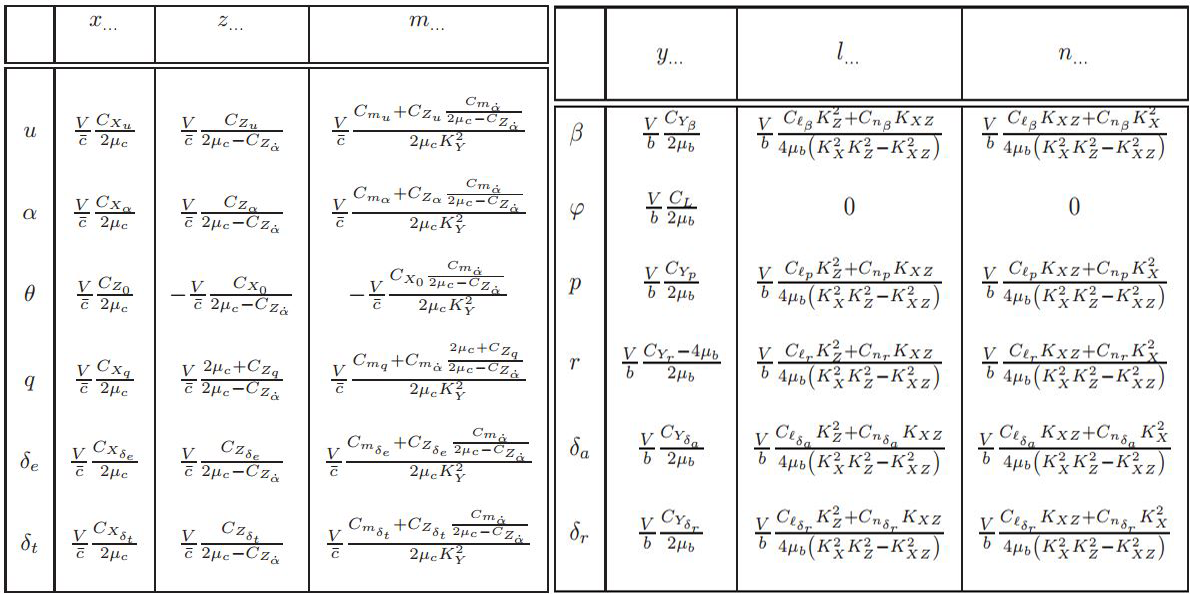
\includegraphics[width=14cm]{figures/tablecomplete.png}
\caption{Coefficient table for the symmetric (left) and the asymmetric (right) modes\cite{fdreader}.}
\label{fig:completetable}
\end{figure}

\begin{figure}
\centering
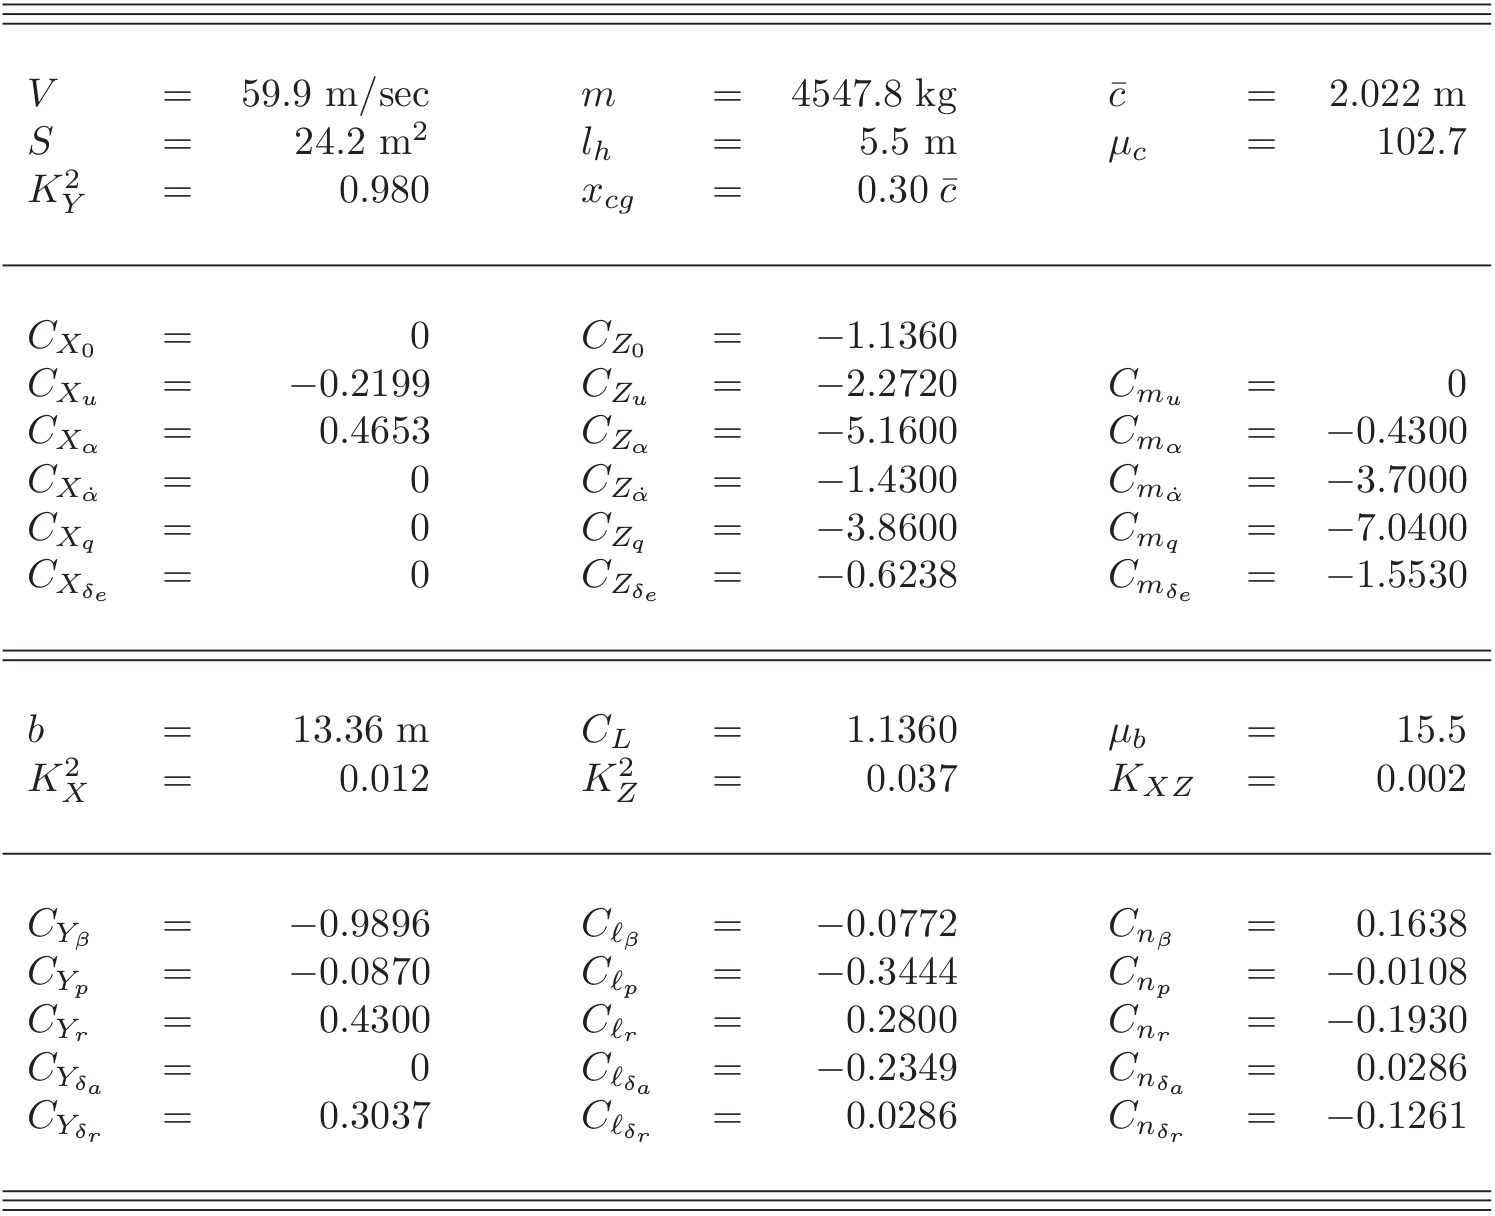
\includegraphics[width=14cm]{figures/tablecoefs.png}
\caption{Symmetric and asymmetric stability and control derivatives for the Cessna Ce500 ‘Citation’, Cruise\cite{fdreader}.}
\label{fig:coeftable}
\end{figure}


A JSBSim input file was manually created with the aerodynamic model given above with the values for the Citation where filled in. The results are shown in Figures~\ref{fig:lti_elevator},~\ref{fig:lti_aileron}~and~\ref{fig:lti_rudder}. As it can be seen the JSBSim and the \gls{lti} system give roughly the same results, specially in the first few simulation seconds. Thus the JSBSim model is deemed good enough to be used to generate test flight data.


\begin{figure}
\centering
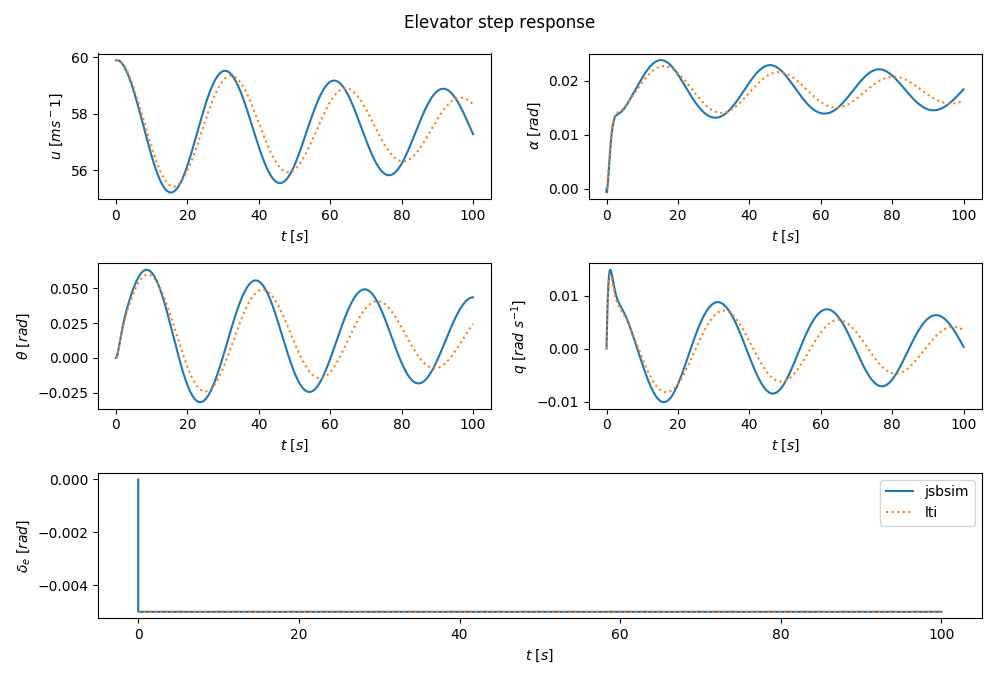
\includegraphics[width=14cm]{figures/lti_elevator}
\caption{Response curves for a step elevator deflection ($\Delta\delta_e=-0.005\ [Rad]$ calculated by JSBSim and the \gls{lti} model.)}
\label{fig:lti_elevator}
\end{figure}

\begin{figure}
\centering
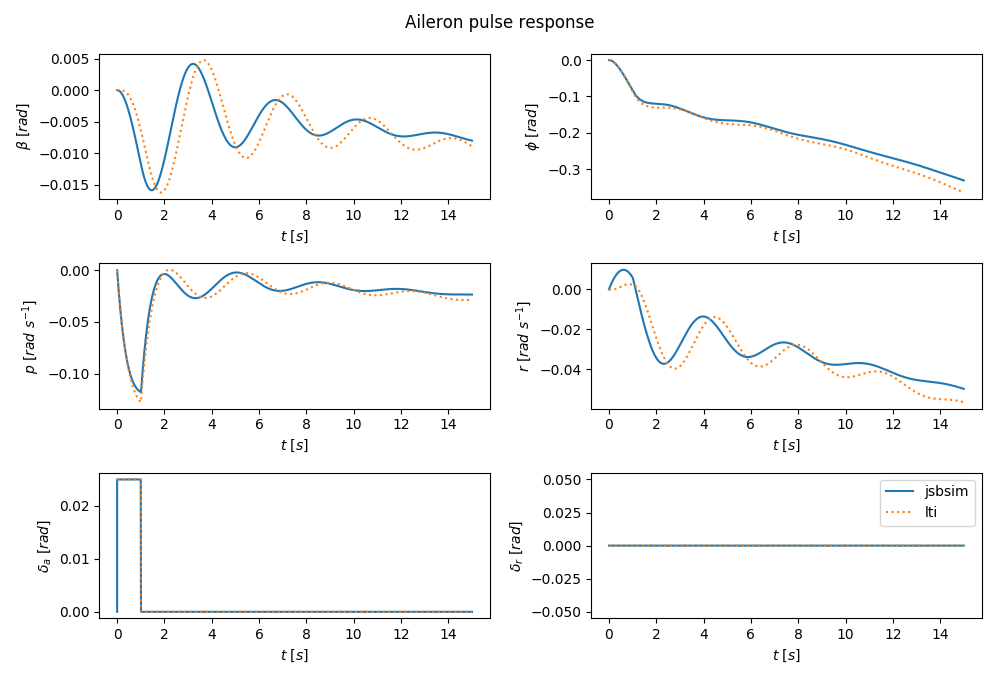
\includegraphics[width=14cm]{figures/lti_aileron}
\caption{Response curves for a pulse shaped aileron deflection ($\Delta\delta_a=0.025\ [Rad]$ calculated by JSBSim and the \gls{lti} model.)}
\label{fig:lti_aileron}
\end{figure}

\begin{figure}
\centering
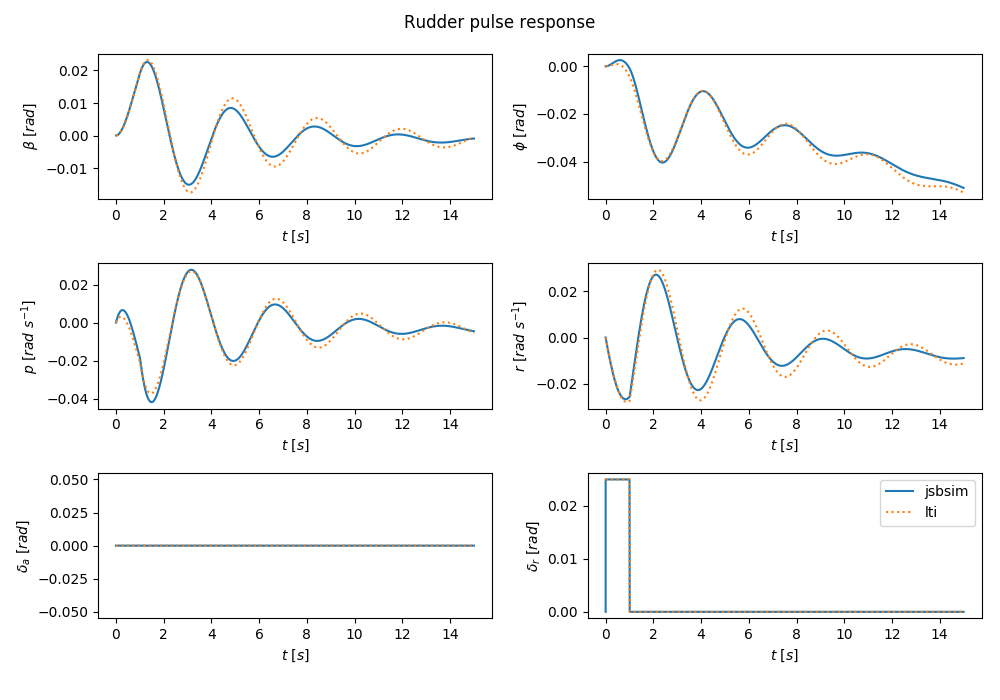
\includegraphics[width=14cm]{figures/lti_rudder}
\caption{Response curves for a pulse shaped rudder deflection ($\Delta\delta_r=0.025\ [Rad]$ calculated by JSBSim and the \gls{lti} model.)}
\label{fig:lti_rudder}
\end{figure}


\subsubsection{Digital Datcom}
Digital Datcom is a program capable of calculating the aerodynamic coefficients using empirical methods contained in the \gls{usaf} Stability and Control Datcom (Data Compendium). The source code for Digital Datcom is available online, however Digital Datcom is written in Fortran. Thus it has been decided to create the Python wrapper around a pre-compiled executable. Datcom+ has thus been chosen. Datcom+ is a modified variant of Digital Datcom which has been extended with extra tools and output formats and is available as a pre-compiled binary file.\\

The Datcom+ wrapper is simple. It consists of a template file with the geometry of the Cessna Ce550 'Citation~II'. The flight conditions and control inputs are left blank since these are filled in by the Python wrapper. This however means that the current wrapper can only generate coefficients for the Citation II. It will thus be necessary to extend this wrapper in the future, but for now it is enough to test and demonstrate the tools being developed.\\

One drawback of Digital Datcom is that not all coefficients can be calculated using it. $C_{X_{\alpha^2}}$ is calculated by fitting a second order polynomial on the value of $C_X$ at different angles of attack. The value of $C_{X_{\alpha^2}}$ will then be the value of the highest order term of the polynomial as it's shown in \autoref{eq:c_x_alpha2}

\begin{equation}
\label{eq:c_x_alpha2}
{C_X}(\alpha ) = {C_{X_{\alpha ^2}}}{\alpha ^2} + {C_{{X_\alpha }}}\alpha  + {C_{{X_0}}}
\end{equation}
 
The rest of the unknown coefficients are either left at zero or a value is chosen such that the resulting model is stable. Keep in mind the goal is to generate aerodynamic models that can be used to test the system identification and coefficient mixing tools and are not required to accurately represent a real aircraft. \\

Since the goal is to simulate an aircraft, more information is needed besides the aerodynamic coefficients. These are the masses, reference area, lengths, etc. most of this information has been collected from 'Jane's All The World's Aircraft: Development \& Production' \cite{janes}. However it was not possible to find a reference containing the \gls{mmoi} for the Citation II. It was thus decided to estimate the \gls{mmoi} using the Class I method described in 'Airplane Design Part V: Component Weight Estimation' by J.~Roskam\cite{roskam_5}. These are Equations~\ref{eq:ros_ixx},~\ref{eq:ros_iyy}~and~\ref{eq:ros_izz}.


\begin{equation}
    \label{eq:ros_ixx}
    {I_{XX}} = {b^2}\bar R_X^2\frac{W}{{4g}}
\end{equation}
\begin{equation}
    \label{eq:ros_iyy}
    {I_{YY}} = {L^2}\bar R_Y^2\frac{W}{{4g}}
\end{equation}
\begin{equation}
    \label{eq:ros_izz}
    {I_{ZZ}} = {e^2}\bar R_Y^2\frac{W}{{4g}}
\end{equation}

Where b and L are the wingspan and overall length of the aircraft and e is given by \autoref{eq:ros_e}.

\begin{equation}
    \label{eq:ros_e}
    e = \frac{{b + L}}{2}
\end{equation}

The non-dimensional radius of gyration $\bar{R}_X$, $\bar{R}_Y$ and $\bar{R}_Z$ tends to be the same for aircraft with the same mission orientation. This assumption is however not necessary in the case of the Citation II, since a table with the non-dimensional radius of gyration is available for this aircraft.\cite{roskam_5}\\

Unfortunately there is no Class I method to determine $J_{XZ}$, thus a Class II analysis is necessary to determine it's value. Since this type of analysis would take to much time and insufficient information on the Citation~II is known, it has been decided to assume a fixed value of $2483.2\ [Kg\ m^2]$. This was calculated by using the same value for $K_{XZ}$ as of the Citation during cruise and then dimensionalize it using the Citation II reference length and mass as shown on \autoref{eq:j_xz}.

\begin{equation}
    \label{eq:j_xz}
    J_{XZ} = K_{XZ} \cdot mb^2
\end{equation}

\subsection{State reconstruction}
As already mentioned, the two step approach has been chosen as the system identification method used to determine the aerodynamic coefficients. The first step is the state reconstruction step. This consists of determining the sate of the aircraft during flight. The reason this is needed is because the onboard sensors contain errors which have to be corrected for and there might be states that are not directly measurable and need to be calculated from the available sensor data. \\

An \gls{iekf} has been chosen as the state estimation algorithm for this first step. The next few sections will give a short explanation into the \gls{kf}, \gls{ekf} and \gls{iekf}.\\

\subsubsection{Kalman Filter}
\label{sssec:kf}
A Kalman Filter is an algorithm that uses a series of measurements containing noise, biases and other errors to create an estimate of unknown variables. These estimates tend to be more accurate than estimates based on single measurements. It does this by making an educated guess of the state on each step based on a known model and mixes it with the measurements using a weighted average that depend on the estimated errors. \\

The \gls{kf} is an optimal linear filter and thus only works with linear systems in form of \autoref{eq:kf}. Where $\dot{\bar x}$ is the state vector, $\bar u $ the input vector, $\bar w$ the system noise, $\bar z$ the measurement vector and $\bar v$ the measurement noise.

\begin{equation}
    \begin{array}{l}
        \dot {\bar x} = A\bar x + B\bar u + G\bar w\\
        \bar z = C\bar x + D\bar u + \bar v
    \end{array}
    \label{eq:kf}
\end{equation}

The \gls{kf} requires a discrete model of the system. Thus the first step is to discretize the system described in \autoref{eq:kf} into \autoref{eq:kfd}\\

\begin{equation}
    \begin{array}{l}
        {{\bar x}_{k + 1}} = {\Phi _{k + 1,k}}{{\bar x}_k} + {\Psi _{k + 1,k}}{{\bar u}_k} + {\Gamma {k + 1,    k}} + {w_{d,k}}\\
        {{\bar z}_{k + 1}} = {H_{k + 1}}{{\bar x}_{k + 1}} + {D_{k + 1}}{{\bar u}_{k + 1}} + {v_{k + 1}}
    \end{array}
    \label{eq:kfd}
\end{equation}

To do this the zero-order hold method is used. This methods assumes a zero-order hold on input $\bar u$ and a continuos integration for the noise $\bar v$. Thus the discrete system can be calculated by the equations shown below.

\begin{equation}
    {\Phi _{k + 1,k}} = {e^{AT}} = {{\cal L}^{ - 1}}{\{ {(sI - A)^{ - 1}}\} _{t = dt}}
\end{equation}

\begin{equation}
    {\Psi _{k + 1,k}} = \left( {\int_{\tau  = 0}^T {{e^{A\tau }}d\tau } } \right)B = {A^{ - 1}}({\Phi_
{k + 1,k}}-I)B
\end{equation}

\begin{equation}
    {\Gamma _{k + 1,k}} = \left( {\int_{\tau  = 0}^T {{e^{A\tau }}d\tau } } \right)G = {A^{ - 1}}({\Phi _{k + 1,k}}-I)G
\end{equation}

\begin{equation}
    {H_{k + 1}} = C
\end{equation}

\begin{equation}
    {D_{k + 1}} = D
\end{equation}

However according to DeCarlo\cite{DeCarlo}, the discrete system with zero-order hold assumptions can be computed using Equations~\ref{eq:di}~and~\ref{eq:dn}. 

\begin{equation}
    {e^{\left[ {\begin{array}{*{20}{c}}
    A&B\\
    0&0
    \end{array}} \right]dt}} = \left[ {\begin{array}{*{20}{c}}
    {{\Phi _{k + 1,k}}}&{{\Psi _{k + 1,k}}}\\
    0&I
    \end{array}} \right]
    \label{eq:di}
\end{equation}

\begin{equation}{e^{\left[ {\begin{array}{*{20}{c}}
    A&G\\
    0&0
    \end{array}} \right]dt}} = \left[ {\begin{array}{*{20}{c}}
    {{\Phi _{k + 1,k}}}&{{\Gamma _{k + 1,k}}}\\
    0&I
    \end{array}} \right]
    \label{eq:dn}
\end{equation}

The basic steps taken in a single \gls{kf} iteration are:
\begin{enumerate}
    \item \textbf{One step ahead prediction}\\
    In this step a prediction of the state vector is made based on the model, the current state estimate and input.  

    \begin{equation}
        {{\hat{\bar x}}_{k + 1,k}} = {\Phi _{k + 1,k}}{{\hat{\bar x}}_{k,k}} + {\Psi _{k + 1,k}}{{\bar u}_k}
    \end{equation}

    \item \textbf{Covariance matrix of state prediction error}\\
    The covariance matrix of the state prediction error is then calculated.

    \begin{equation}
        {P_{k + 1,k}} = {\Phi _{k + 1,k}}{P_k}\Phi _{k + 1,k}^T + {\Gamma _{k + 1,k}}{Q_{d,k}}\Gamma _{k + 1,k}^T
    \end{equation}

    \item \textbf{Kalman gain calculation}\\
    Next the Kalman gain is calculated using \autoref{eq:k_gain}. However during development of the Kalman filter it became came clear that the $({H_{k + 1}}{P_{k + 1,k}}H_{k + 1}^T + {R_{k + 1}})$ term was not always invertible. Thus the Moore-Penrose pseudo-inverse algorithm is used instead. 

    \begin{equation}
        {K_{k + 1}} = {P_{k + 1,k}}H_{k + 1}^T{({H_{k + 1}}{P_{k + 1,k}}H_{k + 1}^T + {R_{k + 1}})^{ - 1}}
        \label{eq:k_gain}
    \end{equation}

    \item \textbf{Measurement update}\\
    In this step the optimal estimate of the states is made. This is done using the following equation.

    \begin{equation}
        {{\hat{\bar x}}_{k + 1,k + 1}} = {{\hat{\bar x}}_{k + 1,k}} + {K_{k + 1}}\left( {{{\bar z}_{k + 1}} - {H_{k + 1}}{{\hat{\bar x}}_{k + 1,k}}} \right)
    \end{equation}

    \item \textbf{Covariance matrix of state estimation error}\\
    The last step is to calculate the covariance matrix of the estimation error that wil be used in the next iteration.

    \begin{equation}
        {P_{k + 1,k + 1}} = \left( {I - {K_{k + 1}}{H_{k + 1}}{{\hat{\bar x}}_{k + 1,k}}} \right)
    \end{equation}
\end{enumerate}


\subsubsection{Extended Kalman Filter}
Since the \gls{kf} can only be applied to linear systems it is not able to handle non-linear systems. The Extended Kalman Filter {\gls{ekf}} extends the \gls{kf} algorithm so that it's able to handle non-linear systems. This is done by modifying the \textit{One-step ahead prediction} and adding two new steps between the \textit{One-step ahead prediction} and \textit{Covariance matrix of state prediction error}. 

The general non-linear state space model is:

\begin{equation}
    \begin{array}{l}
        \dot{\bar x}\left( t \right) = f\left( {\bar x\left( t \right),\bar u\left( t \right),t} \right) + G\left( {\bar x\left( t \right),t} \right)\bar w\\
        {{\bar z}_n}\left( t \right) = h\left( {\bar x\left( t \right),\bar u\left( t \right),t} \right)\\
        \bar z\left( {{t_k}} \right) = {{\bar z}_n}\left( {{t_k}} \right) + \bar v\left( {{t_k}} \right)
        \end{array}
    \label{eq:ekf_form}
\end{equation}

The steps taken during a single \gls{ekf} iteration are described below.

\begin{enumerate}
    \item \textbf{One step ahead prediction}\\
    Since the system is described by a set of non-linear equation, the prediction can be performed using a numerical integrator. In this case a 4th order Runge-Kutta. The process can be described by the equation shown below. 
    \begin{equation}
        {{\hat{\bar x}}_{k + 1,k}} = {{\hat{\bar x}}_{k,k}} + \int_t^{t + dt} f \left( {{{\hat{\bar x}}_{k,k}},{{\bar u}_k},t} \right)dt
    \end{equation}
    \item \textbf{Calculate Jacobians}\\
    Next the system is linearized. This is done by calculating the Jacobian around the the predicted state. The Jacobian matrices are given by.

    \begin{equation}
        {\left. {{F_x}\left( {{{\hat{\bar x}}_{k + 1,k}},{{\bar u}_k},t} \right) = \frac{\delta }{{\delta \bar x}}f\left( {\bar x\left( t \right),\bar u\left( t \right),t} \right)} \right|_{\bar x\left( t \right) = {{\hat {\bar x}}_{k + 1,k}},\bar u\left( t \right) = {{\bar u}_k}}}
    \end{equation}

    \begin{equation}
        {\left. {{H_x}\left( {{{\hat{\bar x}}_{k + 1,k}},{{\bar u}_k},t} \right) = \frac{\delta }{{\delta \bar x}}h\left( {\bar x\left( t \right),\bar u\left( t \right),t} \right)} \right|_{\bar x\left( t \right) = {{\hat{\bar x}}_{k + 1,k}},\bar u\left( t \right) = {{\bar u}_k}}}
    \end{equation}

    The new continuous linear system becomes.


    \begin{equation}
        \begin{gathered}
            \delta \dot{\bar x}\left( t \right) = {F_x}\left( {{{\hat \bar x}_{k + 1,k}},{{\bar u}_k},t} \right)\delta \bar x\left( t \right) + G\left( {\bar x\left( t \right),t} \right)\bar w \hfill \\
            \delta {{\bar z}_n}\left( t \right) = {H_x}\left( {{{\hat \bar x}_{k + 1,k}},{{\bar u}_k},t} \right)\delta \bar x\left( t \right) \hfill \\
            \bar z\left( {{t_k}} \right) = \delta {{\bar z}_n}\left( {{t_k}} \right) + \bar v\left( {{t_k}} \right) \hfill \\ 
          \end{gathered}
    \end{equation}
    \item \textbf{Discretize state transition \& input matrix}\\
    The continues system created in the previous step needs to be converted into a discrete state space system described by \autoref{eq:kfd}. This is done using the same zero-order hold method described in \autoref{sssec:kf}.
    \item \textbf{Covariance matrix of state prediction error}\\
    The covariance matrix of the state prediction error is then calculated in the same way as the \gls{kf}.
    \item \textbf{Kalman gain calculation}\\
    Same as in the previous step, this step is identical to it's counterpart in the \gls{kf}.
    \item \textbf{Measurement update}\\
    This step is almost identical to it's counterpart in the \gls{kf}. The only difference being how the state measurement prediction is calculated.
    \begin{equation}
        {{\hat{\bar x}}_{k + 1,k + 1}} = {{\hat{\bar x}}_{k + 1,k}} + {K_{k + 1}}\left( {{{\bar z}_{k + 1}} - h\left( {{{\hat{\bar x}}_{k + 1,k}},{{\bar u}_k},t} \right)} \right)
    \end{equation}
    \item \textbf{Covariance matrix of state estimation error}\\
    The estimation error covariance matrix is calculated using the following equation.
    \begin{equation}
        {P_{k + 1,k + 1}} = \left( {I - {K_{k + 1}}h\left( {{{\hat{\bar x}}_{k + 1,k}},{{\bar u}_k},t} \right)} \right)
    \end{equation}
\end{enumerate}
\subsubsection{Iterated Extended Kalman Filter}
A limitation of the \gls{ekf} is that it does not guarantee global convergence to it's optimal solution. This is because the \gls{ekf} only uses a first order approximation of the non-linear system and thus the initial condition needs to be close to the optimal solution. Otherwise the \gls{ekf}, might converge slowly or diverge. The Iterated Extended Kalman Filter is an extension to the \gls{ekf} intended to improve the convergence of the \gls{ekf}.\\

For many systems the non-linearities of the observation models are higher than of the dynamic models, the IEKF tries to improve the convergence by using local iterations with new linearizations using new updated state estimates.

The steps taken by the \gls{iekf} are the same as of the \gls{ekf}. The only difference is that steps 2 through 7 are repeated until the change in the estimated state is smaller than some specified value or a maximum number of iterations is reached. The estimated state at the end of iteration 7 is used as the one step ahead prediction in the next one.

\begin{enumerate}
    \item \textbf{One step ahead prediction}\\
    This step is exaclty the same as in the \gls{ekf}.

    \noindent\fbox{%
    \parbox{\textwidth}{%
    \underline{\textbf{Iterative part}}\\
    Before the iteration is stated a new iterator $\eta_i$ is defined. This iterator will contain the state estimate of each iteration $i$. The one-step ahead prediction is set as $\eta_0$, and is thus $\eta_{i-1}$ for the first iteration. Thus the one-step ahead prediction variable ${{\hat{\bar x}}_{k + 1,k}}$ is replaced by $\eta_{i-1}$ on all the steps inside the iterative part.
    \item \textbf{Calculate Jacobians}\\
    \begin{equation}
        {\left. {{F_x}\left( {\eta_{i-1},{{\bar u}_k},t} \right) = \frac{\delta }{{\delta \bar x}}f\left( {\bar x\left( t \right),\bar u\left( t \right),t} \right)} \right|_{\bar x\left( t \right) = \eta_{i-1},\bar u\left( t \right) = {{\bar u}_k}}}
    \end{equation}

    \begin{equation}
        {\left. {{H_x}\left( {\eta_{i-1},{{\bar u}_k},t} \right) = \frac{\delta }{{\delta \bar x}}h\left( {\bar x\left( t \right),\bar u\left( t \right),t} \right)} \right|_{\bar x\left( t \right) = \eta_{i-1},\bar u\left( t \right) = {{\bar u}_k}}}
    \end{equation}
    \item \textbf{Discretize state transition \& input matrix}
    \item \textbf{Kalman gain calculation}
    \item \textbf{Covariance matrix of state prediction error}
    \item \textbf{Measurement update}\\
    The iterative version of the measurement update equation is as following.

    \begin{equation}
        {\eta _i} = {{\hat{\bar x}}_{k + 1,k}} + {K_{k + 1}}\left( {{{\bar z}_{k + 1}} - h\left( {{\eta _{i - 1}},{{\bar u}_k},t} \right) - {H_x}\left( {{{\hat{\bar x}}_{k + 1,k}},{{\bar u}_k},t} \right)\left( {{{\hat{\bar x}}_{k + 1,k}} - {\eta _{i - 1}}} \right)} \right)
    \end{equation}

    \item \textbf{Iteration stop check}\\
    Checks whether the iterative part need to be stopped. As already mentioned there are two conditions under which the iterative part is stopped. The first one being when the changes in the state estimate are smaller than a specified value $\epsilon$ between the last two iterations. Thus this condition is defined by.

    \begin{equation}
        \frac{{\left\| {{\eta _i} - {\eta _{i - 1}}} \right\|}}{{\left\| {{\eta _{i - 1}}} \right\|}} \le \epsilon
    \end{equation}

    The second condition is when a maximum number of iterations has been reached.
    When exiting the loop ${{\hat{\bar x}}_{k + 1,k + 1}}$  is set to equal the last state estimate.

    \begin{equation}
        {{\hat{\bar x}}_{k + 1,k + 1}} = {\eta _i}
    \end{equation}

    }}
    \item \textbf{Covariance matrix of state estimation error}\\
    This step is the same as in the \gls{ekf}.
\end{enumerate}


\subsubsection{IEKF Model}
The model used is largely based on the one from the system identification kalman filter assignment from the TU Delft course \textit{AE4320 System Identification of Aerospace Vehicles}. The state vector $\bar x$, measurement vector $\bar z$, input vector $\bar u$ and system noise input vector $\bar w$ and measurement noise vector $\bar v$ are defined below.


\begin{equation}
    \bar x =  \left [ x, \; y, \; z, \; u, \; v, \; w, \; \phi, \; \theta, \; \psi, \; W_{xe}, \; W_{ye}, \; W_{ze}, \; \lambda_{x}, \; \lambda_{y}, \; \lambda_{z}, \; \lambda_{p}, \; \lambda_{q}, \; \lambda_{r}\right ]
    ^T
\end{equation}

\begin{equation}
    \bar z = \left [ x_{gps_m}, \; y_{gps_m}, \; z_{gps_m}, \; u_{gps_m}, \; v_{gps_m}, \; w_{gps_m}, \; \phi_{gps_m}, \; \theta_{gps_m}, \; \psi_{gps_m}, \; v_{tas_m}, \; \alpha_m, \; \beta_m\right ]
    ^T
\end{equation}

\begin{equation}
    \bar u = \left [ a_{x_m}, \; a_{y_m}, \; a_{z_m}, \; p_{m}, \; q_{m}, \; r_{m}\right ]^T
\end{equation}

\begin{equation}
    \bar w = \left[\begin{matrix}w_{x}, \; w_{y}, \; w_{z}, \; w_{p}, \; w_{q}, \; w_{r}\end{matrix}\right]^T
\end{equation}

\begin{equation}
\bar v = \left[\begin{matrix}v_{x}, \; v_{y}, \; v_{z}, \;  v_u, \; v_v, \; v_w, \; v_\phi, \; v_\theta, \; v_phi, \; v_{vtas}, \; v_\alpha, \; v_\beta \end{matrix}\right]^T
\end{equation}



\autoref{eq:iekf_dyn} defines the dynamic equations of the aircraft. These equations assume that there are no measurement errors in the input, thus the equations need to be modified to include extra bias and noise terms. \autoref{eq:input_error_model} defines the relationship between the the measured accelerations and rotation rates and real accelerations and rotation rates. The $\lambda$ values represent constant biases in the measurements and $w$ are the system noise terms. 

\begin{equation}
    \arraycolsep=1.pt\def\arraystretch{1.5}
    \begin{array}{l}
        \dot x\left( {\bar x,\bar u,t} \right) = {W_{xe}} + \left( {u\cos \left( \theta  \right) + \left( {v\sin \left( \phi  \right) + w\cos \left( \phi  \right)} \right)\sin \left( \theta  \right)} \right)\cos \left( \psi  \right) - \left( {v\cos \left( \phi  \right) - w\sin \left( \phi  \right)} \right)\sin \left( \psi  \right)\\
        \dot y\left( {\bar x,\bar u,t} \right) = {W_{ye}} + \left( {u\cos \left( \theta  \right) + \left( {v\sin \left( \phi  \right) + w\cos \left( \phi  \right)} \right)\sin \left( \theta  \right)} \right)\sin \left( \psi  \right) + \left( {v\cos \left( \phi  \right) - w\sin \left( \phi  \right)} \right)\cos \left( \psi  \right)\\
        \dot z\left( {\bar x,\bar u,t} \right) = {W_{ze}} - u\sin \left( \theta  \right) + \left( {v\sin \left( \phi  \right) + w\cos \left( \phi  \right)} \right)\cos \left( \theta  \right)\\
        \dot u\left( {\bar x,\bar u,t} \right) = {a_x} - g\sin \left( \theta  \right) - qw + rv\\
        \dot v\left( {\bar x,\bar u,t} \right) = {a_y} + g\sin \left( \phi  \right)\cos \left( \theta  \right) + pw - ru\\
        \dot w\left( {\bar x,\bar u,t} \right) = {a_z} + g\cos \left( \phi  \right)\cos \left( \theta  \right) - pv + qu\\
        \dot \phi\left( {\bar x,\bar u,t} \right)  = p + q\sin \left( \phi  \right)\tan \left( \theta  \right) + r\cos \left( \phi  \right)\tan \left( \theta  \right)\\
        \dot \theta\left( {\bar x,\bar u,t} \right)  = q\cos \left( \phi  \right) - r\sin \left( \phi  \right)\\
        \dot \psi\left( {\bar x,\bar u,t} \right)  = q\frac{{\sin \left( \phi  \right)}}{{\cos \left( \theta  \right)}} + r\frac{{\cos \left( \phi  \right)}}{{\cos \left( \theta  \right)}}
        \end{array}
        \label{eq:iekf_dyn}
\end{equation}


\begin{equation}
    \arraycolsep=1.pt\def\arraystretch{1.5}
    \begin{array}{l}
        {a_x} = {a_{{x_m}}} - {\lambda _x} - {w_x}\\
        {a_y} = {a_{{y_m}}} - {\lambda _y} - {w_y}\\
        {a_z} = {a_{{z_m}}} - {\lambda _z} - {w_z}\\
        p = {p_m} - {\lambda _p} - {w_p}\\
        q = {q_m} - {\lambda _q} - {w_q}\\
        r = {r_m} - {\lambda _r} - {w_r}
    \end{array}
    \label{eq:input_error_model}
\end{equation}


Substituting \autoref{eq:input_error_model} into \autoref{eq:iekf_dyn} yields \autoref{eq:iekf_dyn_we}

\begin{equation}
    \arraycolsep=1.pt\def\arraystretch{1.5}
    \begin{array}{*{20}{l}}
        {\dot x = {W_{xe}} + \left( {u\cos \left( \theta  \right) + \left( {v\sin \left( \phi  \right) + w\cos \left( \phi  \right)} \right)\sin \left( \theta  \right)} \right)\cos \left( \psi  \right) - \left( {v\cos \left( \phi  \right) - w\sin \left( \phi  \right)} \right)\sin \left( \psi  \right)}\\
        {\dot y = {W_{ye}} + \left( {u\cos \left( \theta  \right) + \left( {v\sin \left( \phi  \right) + w\cos \left( \phi  \right)} \right)\sin \left( \theta  \right)} \right)\sin \left( \psi  \right) + \left( {v\cos \left( \phi  \right) - w\sin \left( \phi  \right)} \right)\cos \left( \psi  \right)}\\
        {\dot z = {W_{ze}} - u\sin \left( \theta  \right) + \left( {v\sin \left( \phi  \right) + w\cos \left( \phi  \right)} \right)\cos \left( \theta  \right)}\\
        {\dot u = ({a_{{x_m}}} - {\lambda _x} - {w_x}) - g\sin \left( \theta  \right) - ({q_m} - {\lambda _q} - {w_q})w + ({r_m} - {\lambda _r} - {w_r})v}\\
        {\dot v = ({a_{{y_m}}} - {\lambda _y} - {w_y}) + g\sin \left( \phi  \right)\cos \left( \theta  \right) + ({p_m} - {\lambda _p} - {w_p})w - ({r_m} - {\lambda _r} - {w_r})u}\\
        {\dot w = ({a_{{z_m}}} - {\lambda _z} - {w_z}) + g\cos \left( \phi  \right)\cos \left( \theta  \right) - ({p_m} - {\lambda _p} - {w_p})v + ({q_m} - {\lambda _q} - {w_q})u}\\
        {\dot \phi  = ({p_m} - {\lambda _p} - {w_p}) + ({q_m} - {\lambda _q} - {w_q})\sin \left( \phi  \right)\tan \left( \theta  \right) + ({r_m} - {\lambda _r} - {w_r})\cos \left( \phi  \right)\tan \left( \theta  \right)}\\
        {\dot \theta  = ({q_m} - {\lambda _q} - {w_q})\cos \left( \phi  \right) - ({r_m} - {\lambda _r} - {w_r})\sin \left( \phi  \right)}\\
        {\dot \psi  = \frac{{({q_m} - {\lambda _q} - {w_q})\sin \left( \phi  \right)}}{{\cos \left( \theta  \right)}} + \frac{{({r_m} - {\lambda _r} - {w_r})\cos \left( \phi  \right)}}{{\cos \left( \theta  \right)}}}
    \end{array}
    \label{eq:iekf_dyn_we}
\end{equation}

Next a new system of equations is defined with the derivative of the state vector. The the bias terms $\lambda$ and wind are assumed to be constant, thus the derivative of these states is $0$. The new equation is defined at \autoref{eq:iekf_xdot}.


\begin{equation}
    \dot{\bar x} \left( {\bar x,\bar u,t} \right) = \left[ {\begin{array}{*{20}{c}}
        {\dot x\left( {\bar x,\bar u,t} \right)}\\
        {\dot y\left( {\bar x,\bar u,t} \right)}\\
        {\dot z\left( {\bar x,\bar u,t} \right)}\\
        {\dot u\left( {\bar x,\bar u,t} \right)}\\
        {\dot v\left( {\bar x,\bar u,t} \right)}\\
        {\dot w\left( {\bar x,\bar u,t} \right)}\\
        {\dot \phi \left( {\bar x,\bar u,t} \right)}\\
        {\dot \theta \left( {\bar x,\bar u,t} \right)}\\
        {\dot \psi \left( {\bar x,\bar u,t} \right)}\\
        0\\
        0\\
        0\\
        0\\
        0\\
        0\\
        0\\
        0\\
        0
        \end{array}} \right]
        \label{eq:iekf_xdot}
\end{equation}


\autoref{eq:iekf_xdot} needs to be transformed into the same form as \autoref{eq:ekf_form}, to do this the Jacobian of \autoref{eq:iekf_xdot} with respect to the system noise vector $\bar w$ is calculated to get the system noise matrix $G\left( \bullet \right)$. The result is shown in \autoref{eq:iekf_g}. To get the system dynamics equation $f(\bullet)$, the product of the system noise matrix and system noise vector is subtracted from \autoref{eq:iekf_xdot} as shown in \autoref{eq:iekf_f}. 

\begin{equation}
G\left( {\bar x\left( t \right),t} \right) =
\frac{\delta}{\delta \bar w} \dot{\bar x} \left( {\bar x,\bar u,t} \right) = 
\left[\begin{matrix}0 & 0 & 0 & 0 & 0 & 0\\0 & 0 & 0 & 0 & 0 & 0\\0 & 0 & 0 & 0 & 0 & 0\\-1 & 0 & 0 & 0 & w & - v\\0 & -1 & 0 & - w & 0 & u\\0 & 0 & -1 & v & - u & 0\\0 & 0 & 0 & -1 & - \sin{\left (\phi \right )} \tan{\left (\theta \right )} & - \cos{\left (\phi \right )} \tan{\left (\theta \right )}\\0 & 0 & 0 & 0 & - \cos{\left (\phi \right )} & \sin{\left (\phi \right )}\\0 & 0 & 0 & 0 & - \frac{\sin{\left (\phi \right )}}{\cos{\left (\theta \right )}} & - \frac{\cos{\left (\phi \right )}}{\cos{\left (\theta \right )}}\\0 & 0 & 0 & 0 & 0 & 0\\0 & 0 & 0 & 0 & 0 & 0\\0 & 0 & 0 & 0 & 0 & 0\\0 & 0 & 0 & 0 & 0 & 0\\0 & 0 & 0 & 0 & 0 & 0\\0 & 0 & 0 & 0 & 0 & 0\\0 & 0 & 0 & 0 & 0 & 0\\0 & 0 & 0 & 0 & 0 & 0\\0 & 0 & 0 & 0 & 0 & 0\end{matrix}\right]
    \label{eq:iekf_g}
\end{equation}


\begin{equation}
    \arraycolsep=1.pt\def\arraystretch{1.5}
    f\left(\bar x, \bar u, t \right ) = 
    \dot{\bar x}\left( {\bar x,\bar u,t} \right) - G\left( {\bar x,\bar u,t} \right)\bar w =     
\left[\begin{matrix}W_{xe} + \left(u \cos{\left (\theta \right )} + \left(v \sin{\left (\phi \right )} + w \cos{\left (\phi \right )}\right) \sin{\left (\theta \right )}\right) \cos{\left (\psi \right )} - \left(v \cos{\left (\phi \right )} - w \sin{\left (\phi \right )}\right) \sin{\left (\psi \right )}\\
W_{ye} + \left(u \cos{\left (\theta \right )} + \left(v \sin{\left (\phi \right )} + w \cos{\left (\phi \right )}\right) \sin{\left (\theta \right )}\right) \sin{\left (\psi \right )} + \left(v \cos{\left (\phi \right )} - w \sin{\left (\phi \right )}\right) \cos{\left (\psi \right )}\\
W_{ze} - u \sin{\left (\theta \right )} + \left(v \sin{\left (\phi \right )} + w \cos{\left (\phi \right )}\right) \cos{\left (\theta \right )}\\
a_{x_m} - \lambda_{x} + v \left(- \lambda_{r} + r_{m}\right) + w \left(\lambda_{q} - q_{m}\right) - g \sin{\left (\theta \right )}\\a_{y_m} - \lambda_{y} + u \left(\lambda_{r} - r_{m}\right) + w \left(- \lambda_{p} + p_{m}\right) + g \sin{\left (\phi \right )} \cos{\left (\theta \right )}\\
a_{z_m} - \lambda_{z} + u \left(- \lambda_{q} + q_{m}\right) + v \left(\lambda_{p} - p_{m}\right) + g \cos{\left (\phi \right )} \cos{\left (\theta \right )}\\
- \lambda_{p} - \lambda_{q} \sin{\left (\phi \right )} \tan{\left (\theta \right )} - \lambda_{r} \cos{\left (\phi \right )} \tan{\left (\theta \right )} + p_{m} + q_{m} \sin{\left (\phi \right )} \tan{\left (\theta \right )} + r_{m} \cos{\left (\phi \right )} \tan{\left (\theta \right )}\\
- \lambda_{q} \cos{\left (\phi \right )} + \lambda_{r} \sin{\left (\phi \right )} + q_{m} \cos{\left (\phi \right )} - r_{m} \sin{\left (\phi \right )}\\
\frac{1}{\cos{\left (\theta \right )}} \left(- \lambda_{q} \sin{\left (\phi \right )} - \lambda_{r} \cos{\left (\phi \right )} + q_{m} \sin{\left (\phi \right )} + r_{m} \cos{\left (\phi \right )}\right)\\

0\\0\\0\\0\\0\\0\\0\\0\\0\end{matrix}\right]
\label{eq:iekf_f}
\end{equation}

The observation model including the measurement noise $v$ are shown in \autoref{eq:obs_model}. To transform \autoref{eq:obs_model} into the same form as \autoref{eq:ekf_form}, the observation equation $h(\bullet)$ is defined in 

\begin{equation}
    \arraycolsep=1.pt\def\arraystretch{1.5}
    \begin{array}{l}
    {x_{gp{s_m}}} = x + {v_x}\\
    {y_{gp{s_m}}} = y + {v_y}\\
    {z_{gp{s_m}}} = z + {v_z}\\
    {u_{gp{s_m}}} = {W_{xe}} + \left( {u\cos \left( \theta  \right) + \left( {v\sin \left( \phi  \right) + w\cos \left( \phi  \right)} \right)\sin \left( \theta  \right)} \right)\cos \left( \psi  \right) - \left( {v\cos \left( \phi  \right) - w\sin \left( \phi  \right)} \right)\sin \left( \psi  \right) + {v_u}\\
    {v_{gp{s_m}}} = {W_{ye}} + \left( {u\cos \left( \theta  \right) + \left( {v\sin \left( \phi  \right) + w\cos \left( \phi  \right)} \right)\sin \left( \theta  \right)} \right)\sin \left( \psi  \right) + \left( {v\cos \left( \phi  \right) - w\sin \left( \phi  \right)} \right)\cos \left( \psi  \right) + {v_v}\\
    {w_{gp{s_m}}} = {W_{ye}} + \left( {u\cos \left( \theta  \right) + \left( {v\sin \left( \phi  \right) + w\cos \left( \phi  \right)} \right)\sin \left( \theta  \right)} \right)\sin \left( \psi  \right) + \left( {v\cos \left( \phi  \right) - w\sin \left( \phi  \right)} \right)\cos \left( \psi  \right) + {v_w}\\
    {\phi _{gp{s_m}}} = \phi  + {v_\phi }\\
    {\theta _{gp{s_m}}} = \theta  + {v_\theta }\\
    {\psi _{gp{s_m}}} = \psi  + {v_\psi }\\
    {V_{ta{s_m}}} = \sqrt {{u^2} + {v^2} + {w^2}}  + {v_{vtas}}\\
    {\alpha _m} = {\mathop{\rm atan}\nolimits} \left( {\frac{w}{u}} \right) + {v_\alpha }\\
    {\beta _m} = {\mathop{\rm atan}\nolimits} \left( {\frac{v}{{\sqrt {{u^2} + {w^2}} }}} \right) + {v_\beta }
    \end{array} 
    \label{eq:obs_model}
\end{equation}


\begin{equation}
    h\left(\bar x, \bar u, t \right ) =
    \left[ {\begin{array}{*{20}{c}}
        x\\
        y\\
        z\\
        {{W_{xe}} + \left( {u\cos \left( \theta  \right) + \left( {v\sin \left( \phi  \right) + w\cos \left( \phi  \right)} \right)\sin \left( \theta  \right)} \right)\cos \left( \psi  \right) - \left( {v\cos \left( \phi  \right) - w\sin \left( \phi  \right)} \right)\sin \left( \psi  \right)}\\
        {{W_{ye}} + \left( {u\cos \left( \theta  \right) + \left( {v\sin \left( \phi  \right) + w\cos \left( \phi  \right)} \right)\sin \left( \theta  \right)} \right)\sin \left( \psi  \right) + \left( {v\cos \left( \phi  \right) - w\sin \left( \phi  \right)} \right)\cos \left( \psi  \right)}\\
        {{W_{ze}} - u\sin \left( \theta  \right) + \left( {v\sin \left( \phi  \right) + w\cos \left( \phi  \right)} \right)\cos \left( \theta  \right)}\\
        \phi \\
        \theta \\
        \psi \\
        {\sqrt {{u^2} + {v^2} + {w^2}} }\\
        {{\mathop{\rm atan}\nolimits} \left( {\frac{w}{u}} \right)}\\
        {{\mathop{\rm atan}\nolimits} \left( {\frac{v}{{\sqrt {{u^2} + {w^2}} }}} \right)}
        \end{array}} \right]
        \label{eq:iekf_h}
\end{equation}

The \gls{ekf} and \gls{iekf} require the Jacobian matrices of \autoref{eq:iekf_f} and \autoref{eq:iekf_h}. These matrices are generated during the script initialization process by means of symbolic computations using sympy.


\subsubsection{Testing IEKF}
The IEKF python module that was developed is unit-tested using smaller non-linear models with fewer states and inputs. These tests show that the IEKF algorithm was implemented properly. The results of one of these test are shown below.\\

The test system has two states, two inputs and one measurement. The state, input and measurement vectors and the system, observation and noise input equations are shown from Equations~\ref{eq:wlke}~to~\ref{eq:ksd}. As already mentioned, the Jacobian matrices are calculated during initialization using symbolic computations.\\ 

\begin{equation}
    \bar x = \left [ x_{1}, \; x_{2}\right ]
    \label{eq:wlke}
\end{equation}
\begin{equation}
    \bar u = \left [ u_{1}, \; u_{2}\right ]
\end{equation}
\begin{equation}
    \bar z = \left [ z_{1} \right]
\end{equation}
\begin{equation}
    f\left(\bar x, \bar u, t \right ) = 
    \left[\begin{matrix}u_{1} + x_{2} \cos^{3}{\left (x_{1} \right )}\\u_{2} - x_{2}\end{matrix}\right]
\end{equation}
\begin{equation}
    G\left(\bar x, \bar u, t \right ) = 
    \left[\begin{matrix}1.0 & 0.0\\0.0 & 1.0\end{matrix}\right]
\end{equation}
\begin{equation}
    h\left(\bar x, \bar u, t \right ) = 
    \left[\begin{matrix}u_{1} x_{2}^{2} + x_{1}^{2}\end{matrix}\right]
    \label{eq:ksd}
\end{equation}

The test data was simulated using the same model. The standard deviation of the two system noise sources are $[2, 1]$. The measurement noise standard deviation is $3$. The simulation initial states are $[2.0, -3.0]$ and the initial states given to the filter are $[10.0, 1.0]$. The initial covariance matrix of estimatation error is a $2x2$ diagonal matrix with $100$ in the diagonal elements. The results of this test are shown in \autoref{fig:iekf_test}.

\begin{figure}
    \centering
    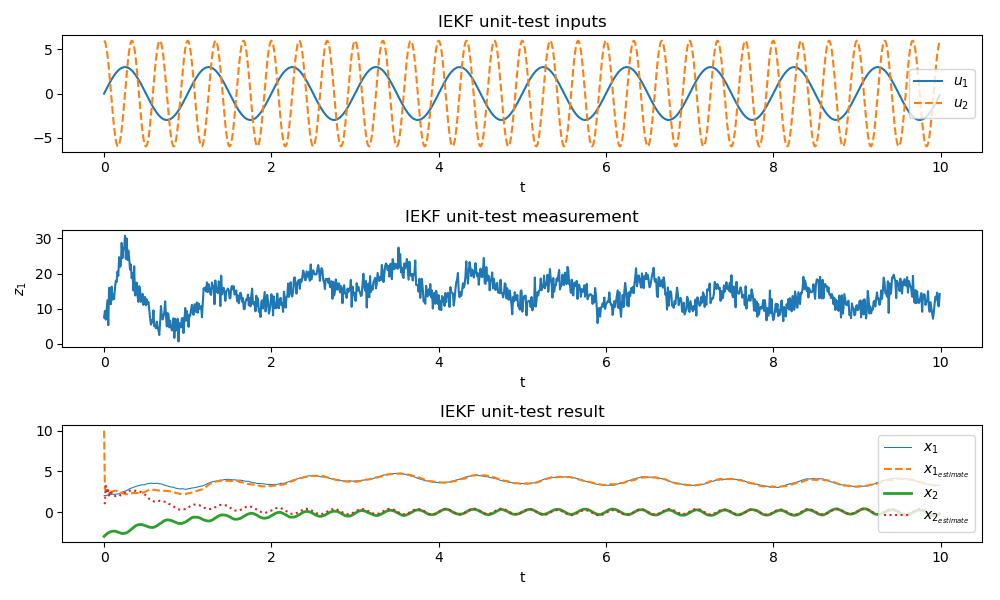
\includegraphics[width=14cm]{figures/iekf_test}
    \caption{Elevator deflection during the 3211 manoeuvre.}
    \label{fig:iekf_test}
\end{figure}


To test the aircarft model derived in the previous section the data provided with the \textit{AE4320 System Identification of Aerospace Vehicles} assignment is used.\\

For this test the accelerometer biases where set to $0.001~[m\;s^{-2}]$, gyro biases $0.001~[deg\;s^{-1}]$, gps position standard deviation to $10\;[m]$, gps velocity standard deviation to $0.1~[m\;s^{-1}]$, gps orientation standard deviation to $0.1~[rad]$, true airspeed standard deviation to $0.1~[m\;s^{-1}]$ and angle of attack and slide-slip angle standard deviations to $0.1~[deg]$.\\


\begin{figure}
    \centering
    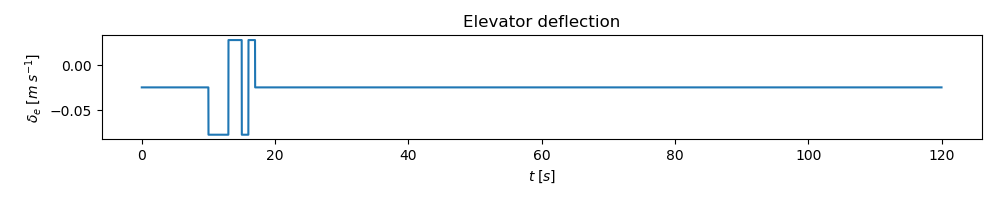
\includegraphics[width=14cm]{figures/iekf_de}
    \caption{Elevator deflection during the 3211 manoeuvre.}
    \label{fig:iekf_de}
\end{figure}

\begin{figure}
    \centering
    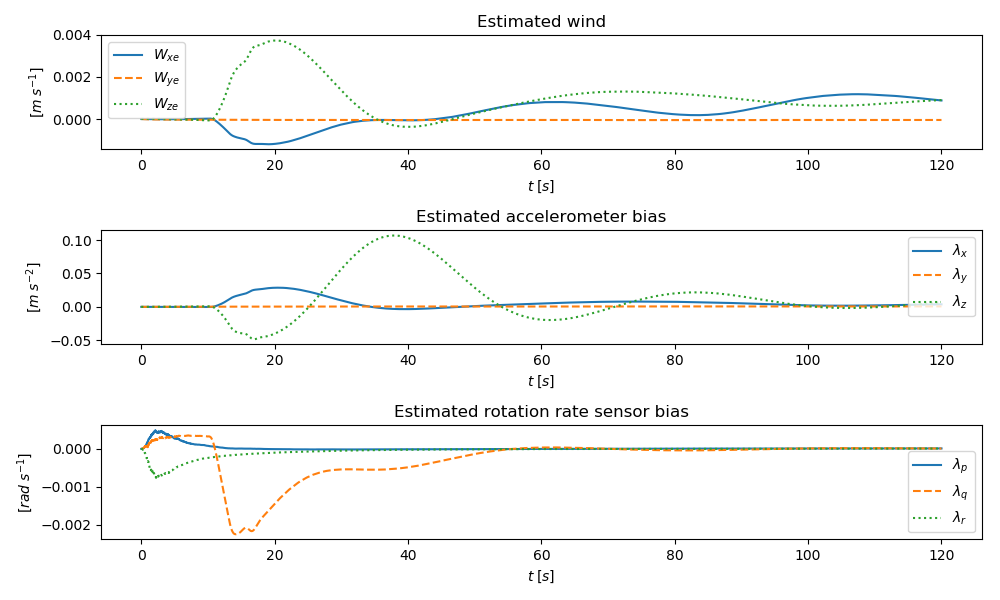
\includegraphics[width=14cm]{figures/iekf_wag}
    \caption{Estimated wind velocities and sensor biases during the 3211 manoeuvre.}
    \label{fig:iekf_wag}
\end{figure}

\begin{figure}
    \centering
    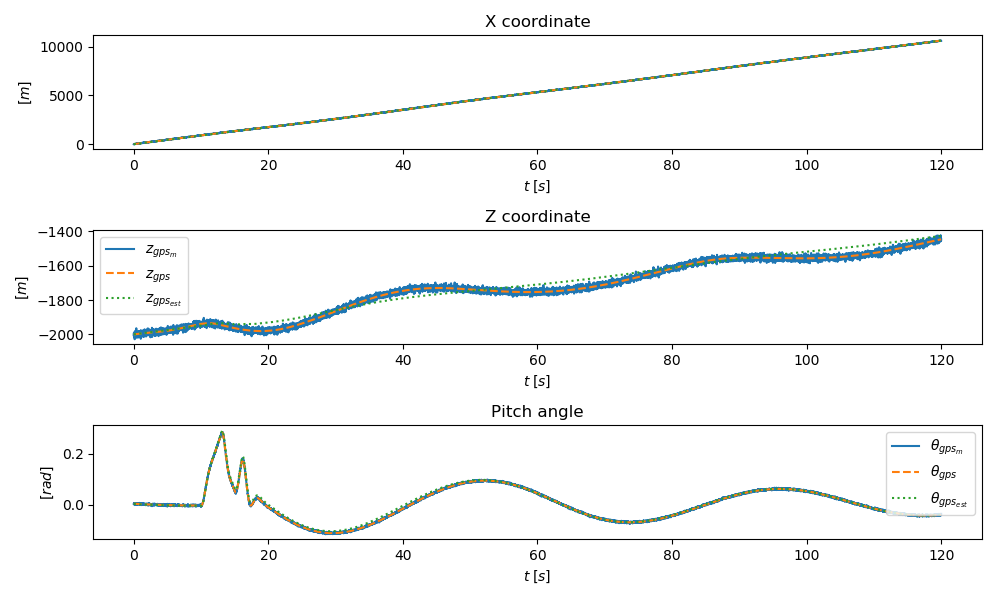
\includegraphics[width=14cm]{figures/iekf_xzphi}
    \caption{Estimated wind velocities and sensor biases.}
    \label{fig:iekf_xzphi}
\end{figure}

As it can be seen the \gls{iekf} is able to correctly estimate the X-coordinate and pitch angle. However the rest of the plots show that the filter is not working properly. The wind and sensor bias estimates are not converging and the Z-coordinate estimate is being smoothed to much. The cause of the errors could be due to errors in the derivation of the model, initial state or initial covariance matrix of state estimation error.































